\chapter{Additional Model Results}
\label{appn:modelresults}

\section{Verification Plots for Poor Performing Models}

\subsection{Storm Maximum Intensity First Points Only}

\begin{figure}[h]
    \centering
    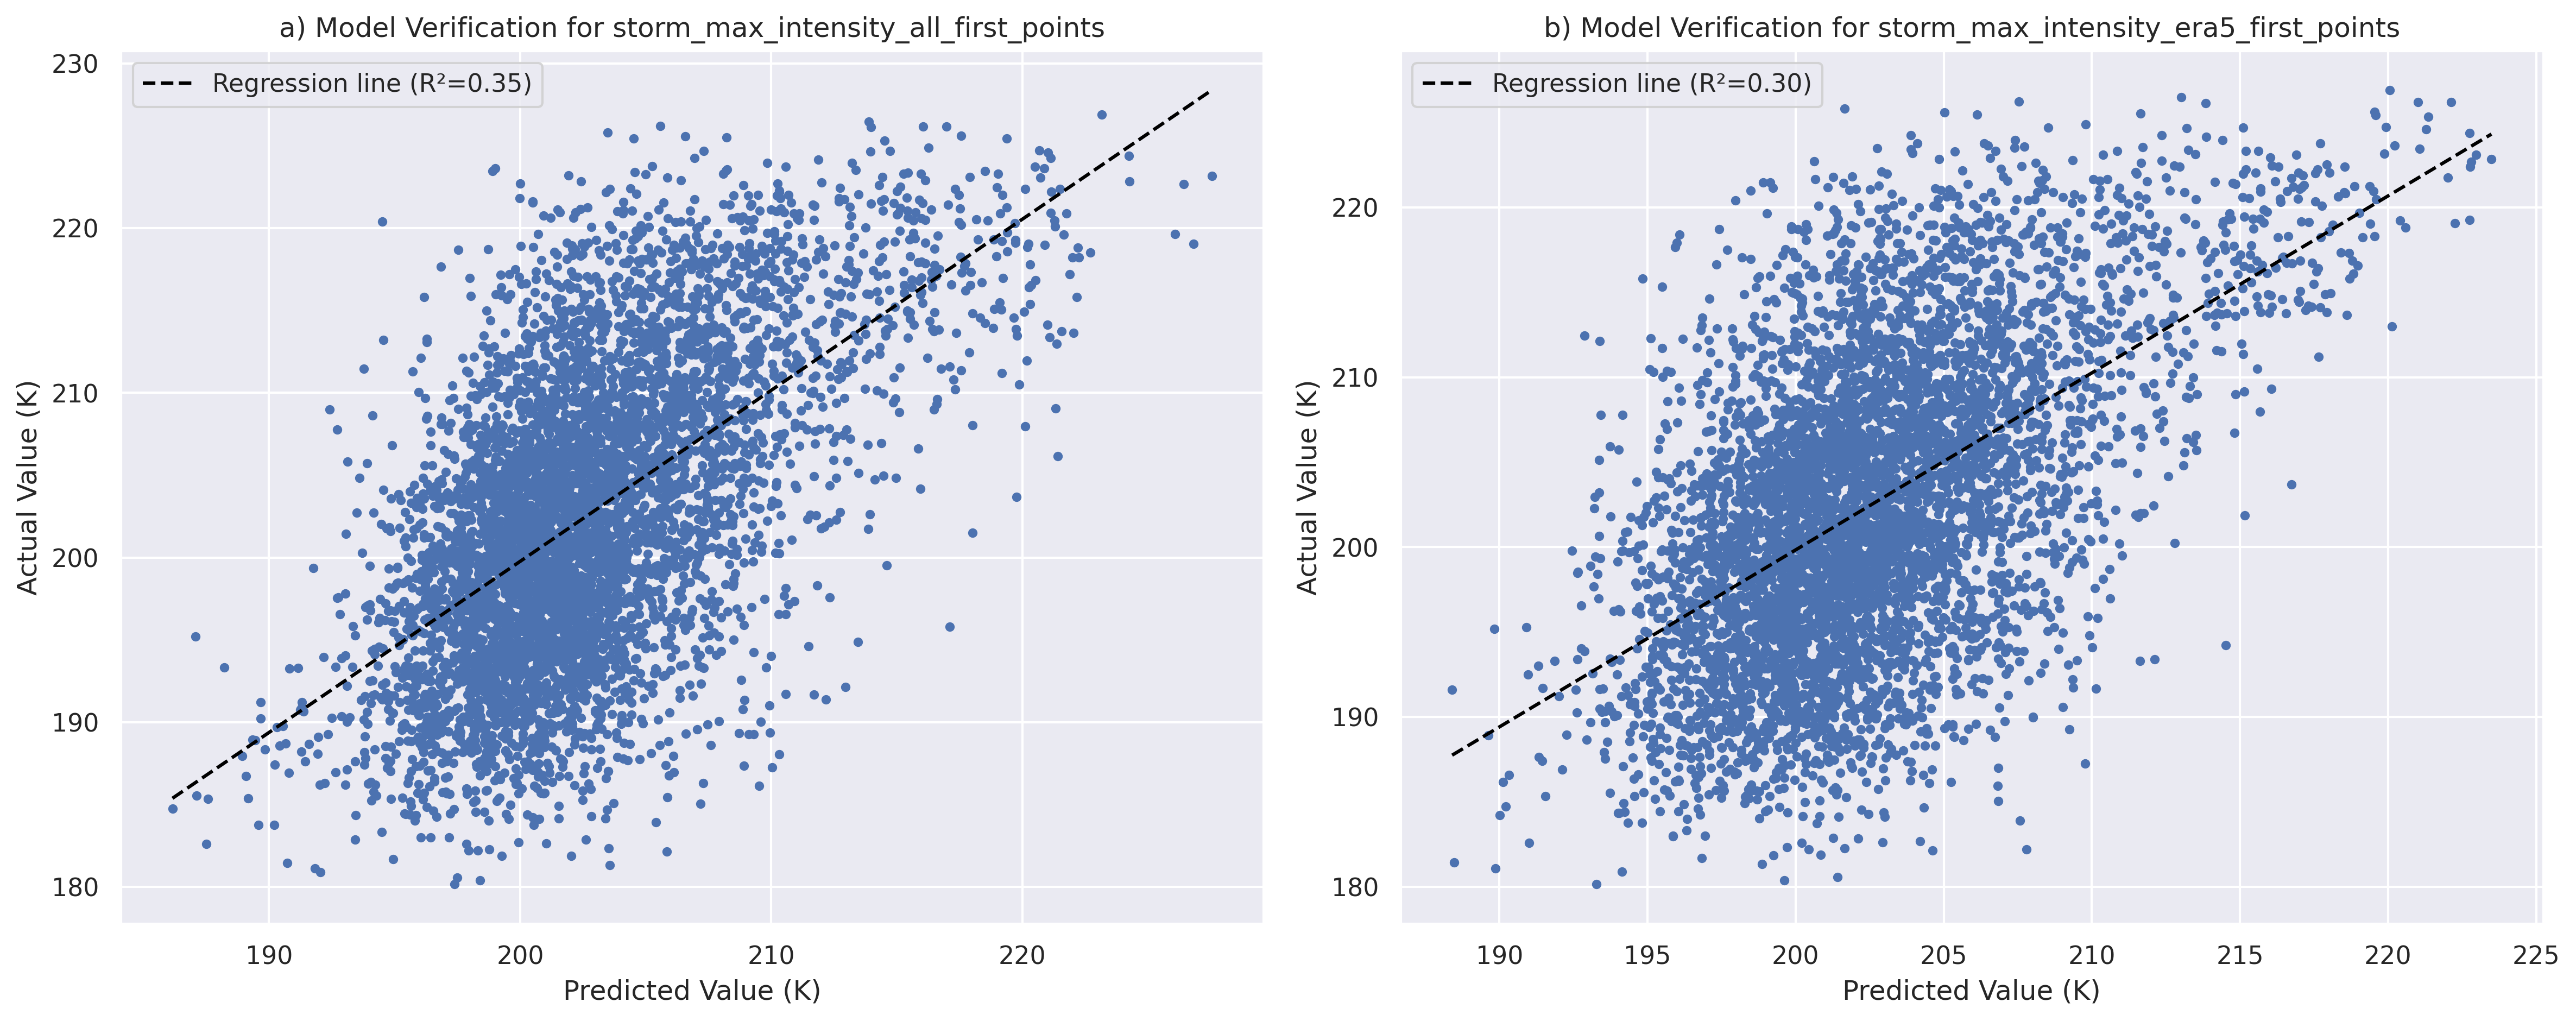
\includegraphics[width=\textwidth]{../figures/generated/experiments/storm_max_intensity_first_points/storm_max_intensity_first_points_summary.png}
    \caption{Comparison of performance and top features for storm maximum intensity (First Points Only).}
    \label{fig:storm_max_intensity_first_points_summary}
\end{figure}

\subsubsection{Storm Direction First Points Only}

\begin{figure}[h]
    \centering
    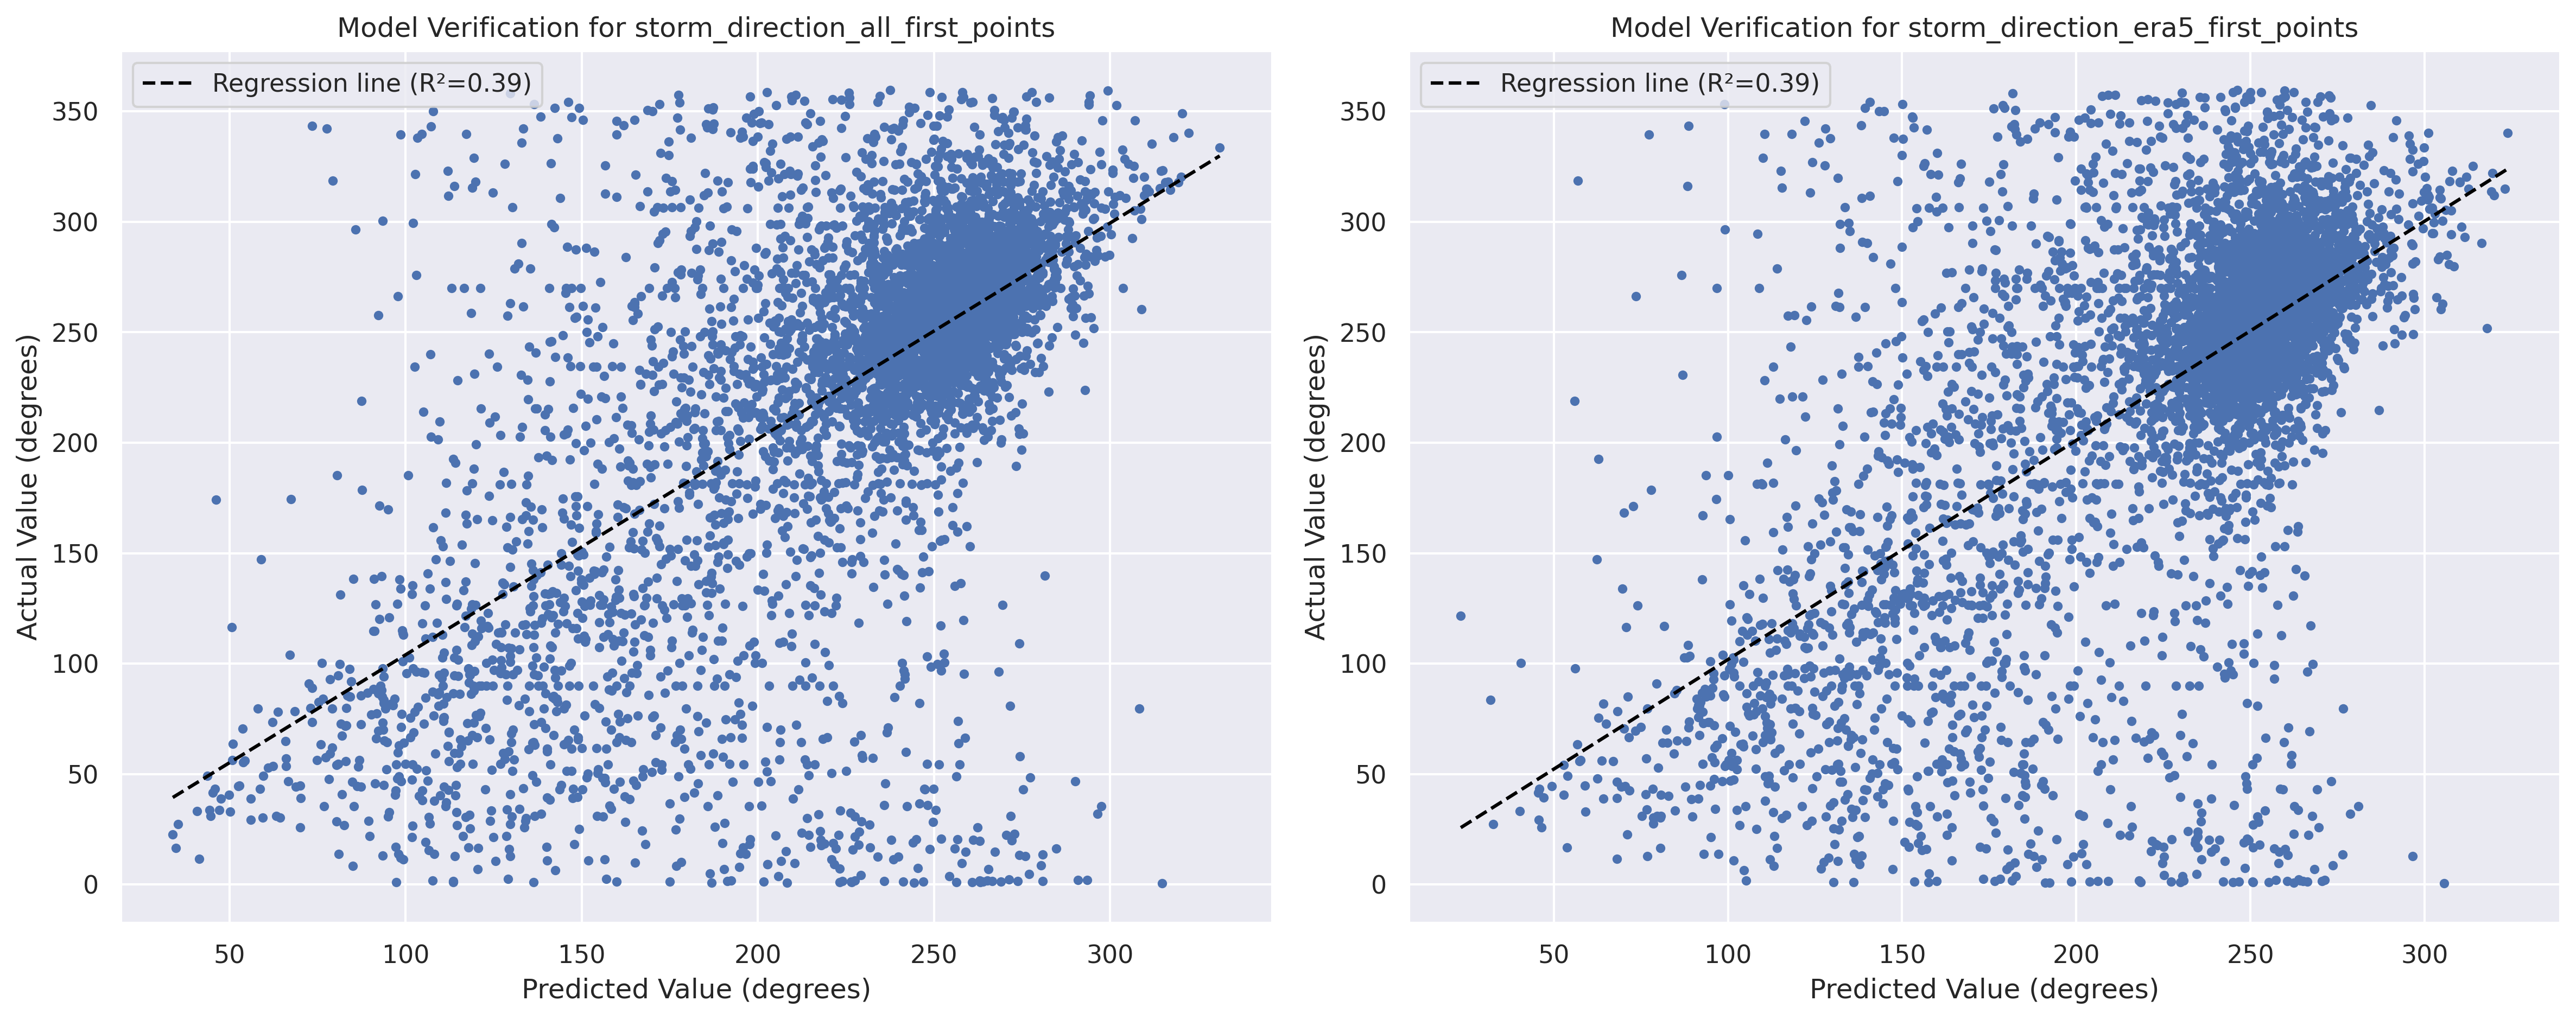
\includegraphics[width=\textwidth]{../figures/generated/experiments/storm_direction_first_points/storm_direction_first_points_summary.png}
    \caption{Comparison of performance and top features for storm direction (First Points Only).}
    \label{fig:storm_direction_first_points_summary}
\end{figure}

\subsection{Next Direction}

\begin{figure}[ht]
    \centering
    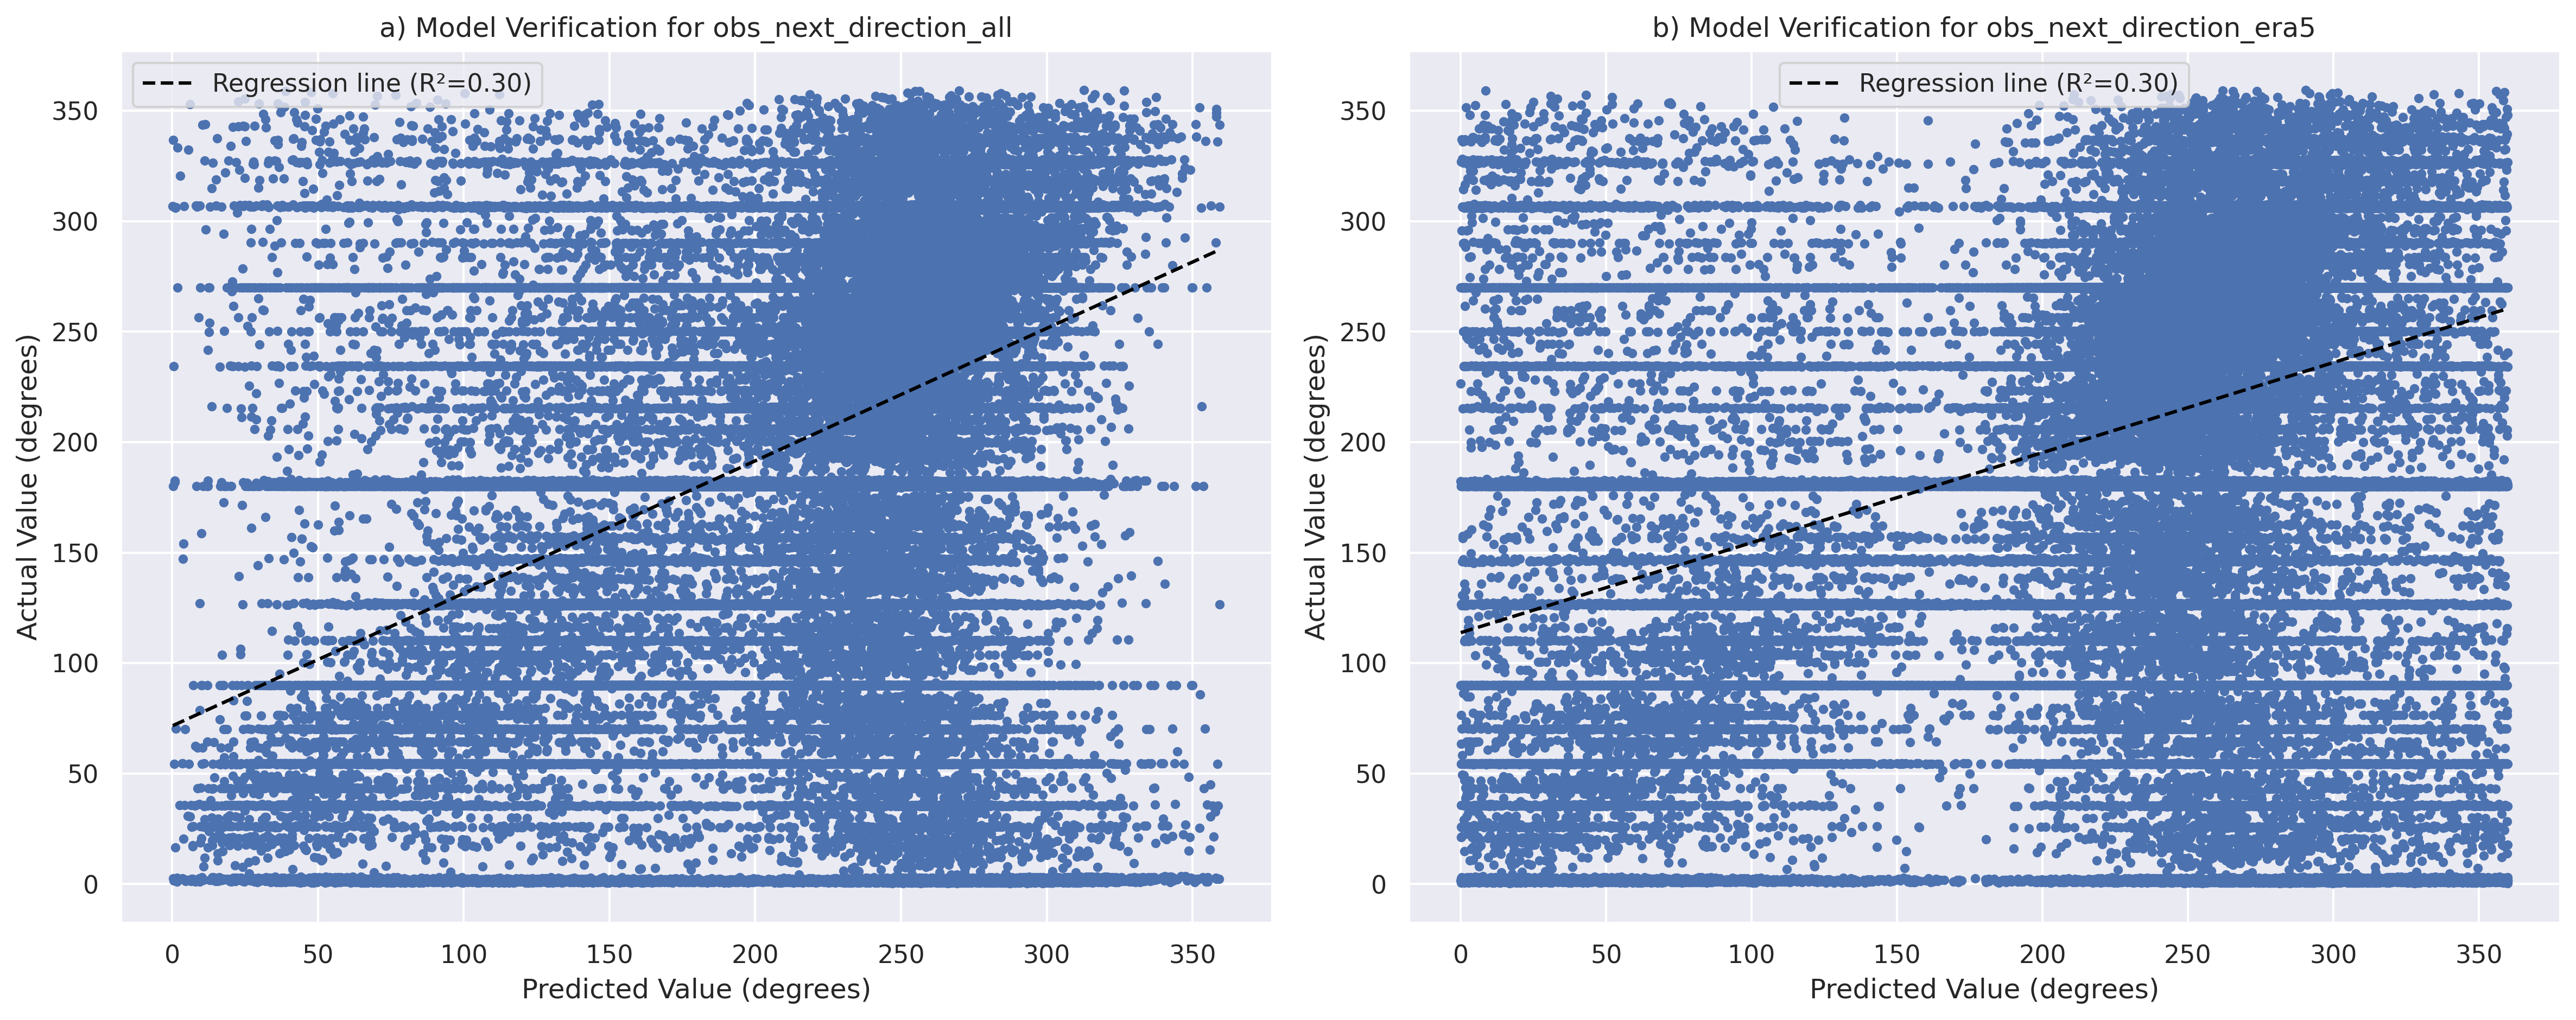
\includegraphics[width=\textwidth]{../figures/generated/experiments/obs_next_direction/obs_next_direction_summary.png}
    \caption{Comparison of performance and top features for next direction.}
    \label{fig:obs_direction_summary}
\end{figure}

\subsection{Next Distance}

\begin{figure}[ht]
    \centering
    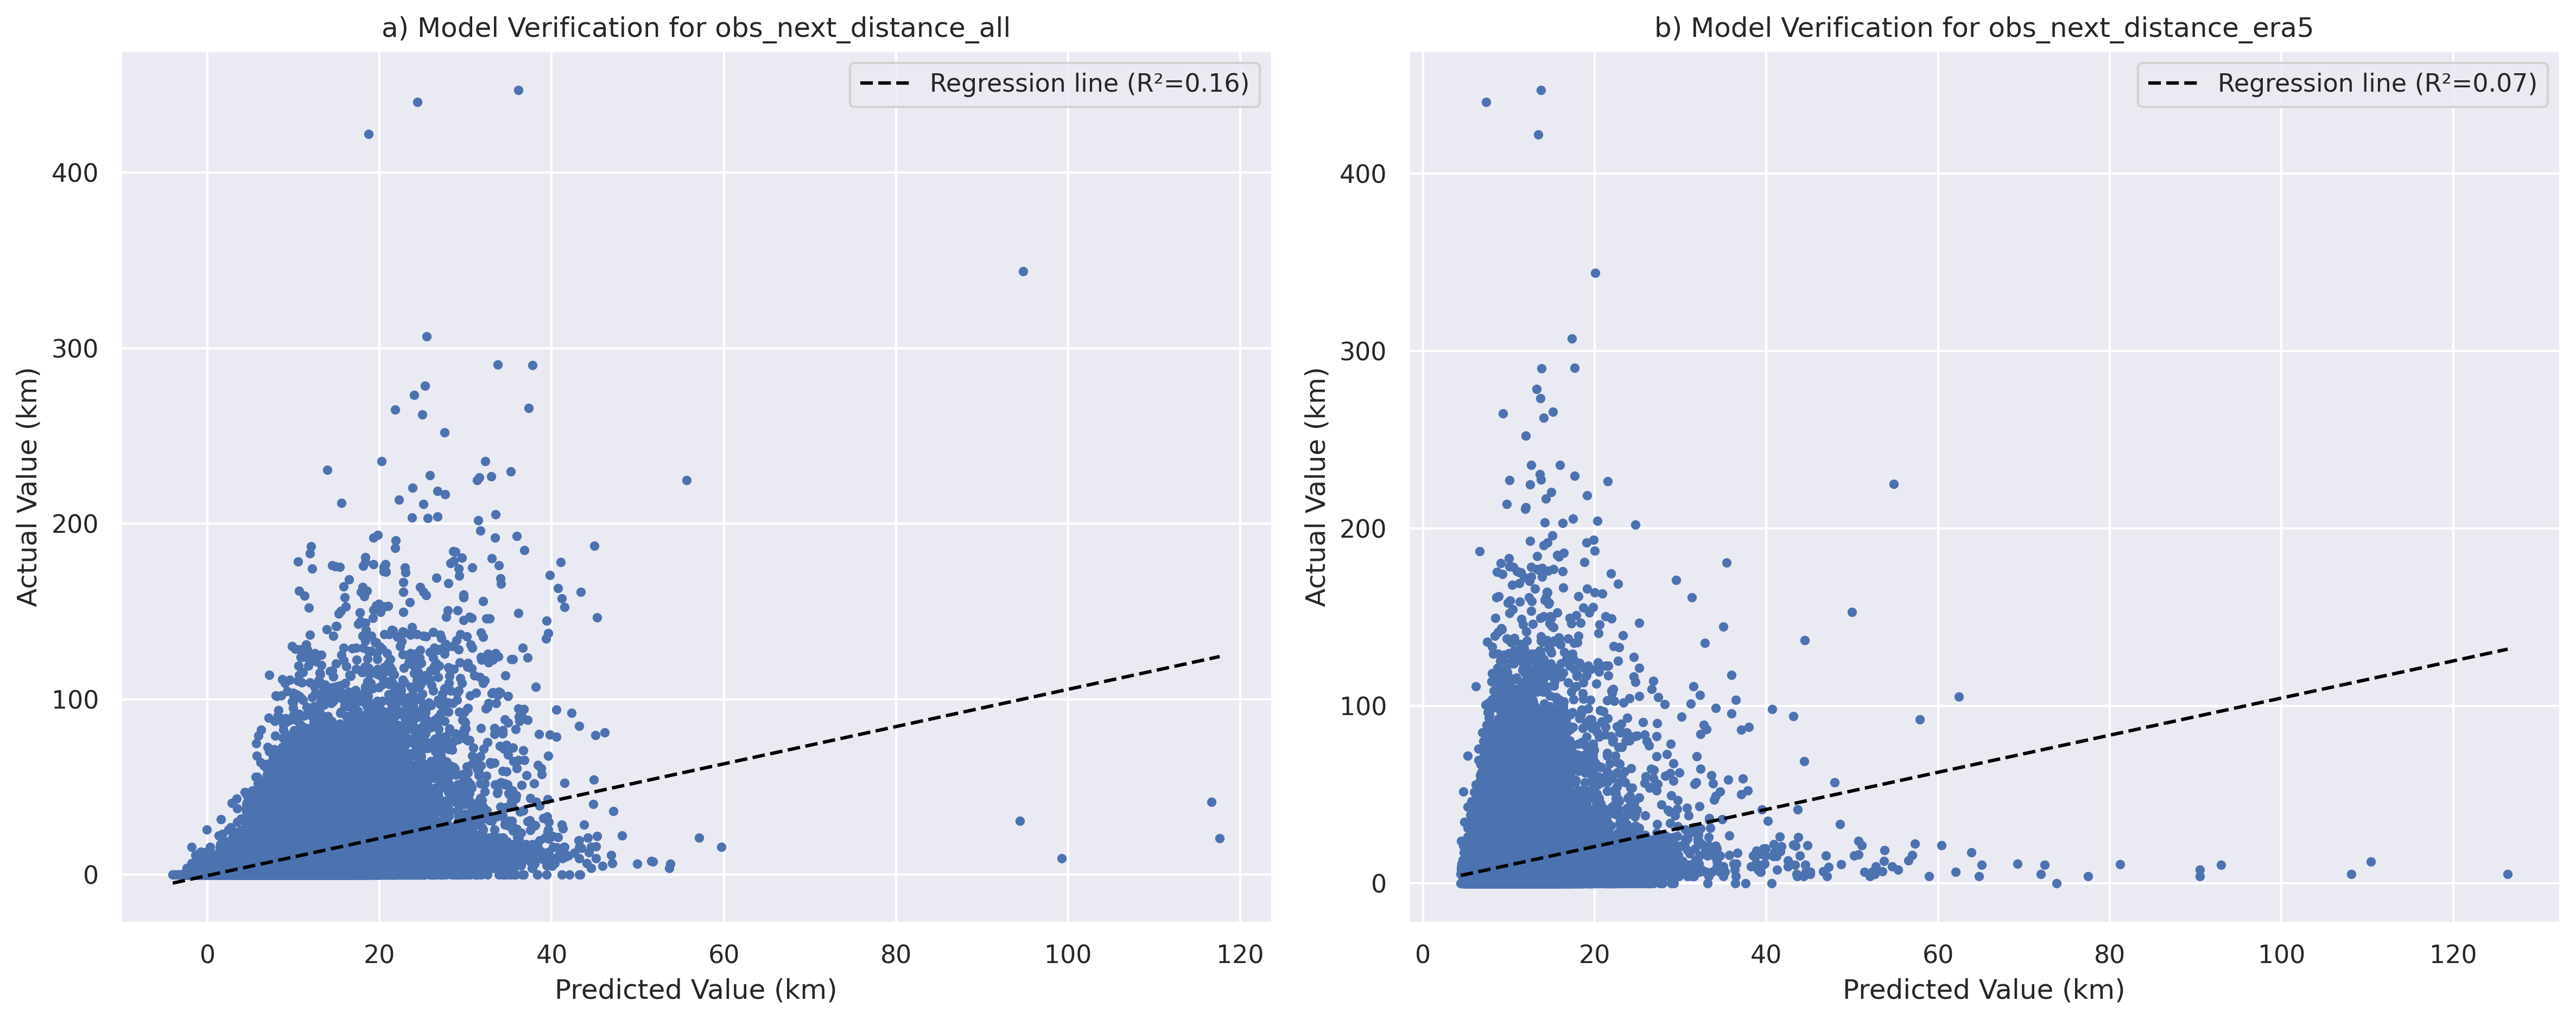
\includegraphics[width=\textwidth]{../figures/generated/experiments/obs_next_distance/obs_next_distance_summary.png}
    \caption{Comparison of performance and top features for next distance.}
    \label{fig:obs_distance_summary}
\end{figure}